\documentclass{emulateapj}
\submitted{{\it Submitted for publication in ApJ}}
\usepackage{multirow,color,wrapfig,ulem}
\usepackage {graphicx}
\usepackage{graphics}
\usepackage[dvips]{epsfig}

%=========================================================================
%		INTERNAL MACROS
%=========================================================================

\newcommand{\avg}[1]{\langle{#1}\rangle}  

\newcommand{\LCDM}{$\Lambda$CDM~}
\newcommand{\beq}{\begin{eqnarray}}  
\newcommand{\eeq}{\end{eqnarray}}  
\newcommand{\zz}{$z\sim 3$} 

\newcommand{\ly}{{\ifmmode{{\rm Ly}\alpha}\else{Ly$\alpha$}\fi}}
\newcommand{\hMpc}{{\ifmmode{h^{-1}{\rm Mpc}}\else{$h^{-1}$Mpc}\fi}}  
\newcommand{\hGpc}{{\ifmmode{h^{-1}{\rm Gpc}}\else{$h^{-1}$Gpc}\fi}}  
\newcommand{\hmpc}{{\ifmmode{h^{-1}{\rm Mpc}}\else{$h^{-1}$Mpc}\fi}}  
\newcommand{\hkpc}{{\ifmmode{h^{-1}{\rm kpc}}\else{$h^{-1}$kpc}\fi}}  
\newcommand{\hMsun}{{\ifmmode{h^{-1}{\rm {M_{\odot}}}}\else{$h^{-1}{\rm{M_{\odot}}}$}\fi}}  
\newcommand{\hmsun}{{\ifmmode{h^{-1}{\rm {M_{\odot}}}}\else{$h^{-1}{\rm{M_{\odot}}}$}\fi}}  
\newcommand{\Msun}{{\ifmmode{{\rm {M_{\odot}}}}\else{${\rm{M_{\odot}}}$}\fi}}  
\newcommand{\msun}{{\ifmmode{{\rm {M_{\odot}}}}\else{${\rm{M_{\odot}}}$}\fi}}  
\newcommand{\lya}{{Lyman$\alpha$~}}
\newcommand{\clara}{{\texttt{CLARA}}~}
\newcommand{\rand}{{\ifmmode{{\mathcal{R}}}\else{${\mathcal{R}}$ }\fi}}  
%SAMPLES
\newcommand{\GHBDM}{\texttt{GH}$_{\mbox{\tiny{BDM}}}$ }
\newcommand{\GHFOF}{\texttt{GH}$_{\mbox{\tiny{FOF}}}$ }
\newcommand{\IHBDM}{\texttt{IH}$_{\mbox{\tiny{BDM}}}$ }
\newcommand{\IHFOF}{\texttt{IH}$_{\mbox{\tiny{FOF}}}$ }
\newcommand{\PBDM}{\texttt{P}$_{\mbox{\tiny{BDM}}}$ }
\newcommand{\PFOF}{\texttt{P}$_{\mbox{\tiny{FOF}}}$ }
\newcommand{\IPBDM}{\texttt{IP}$_{\mbox{\tiny{BDM}}}$ }
\newcommand{\IPFOF}{\texttt{IP}$_{\mbox{\tiny{FOF}}}$ }
\newcommand{\RIPBDM}{\texttt{RIP}$_{\mbox{\tiny{BDM}}}$ }
\newcommand{\RIPFOF}{\texttt{RIP}$_{\mbox{\tiny{FOF}}}$ }


%MY COMMANDS #############################################################
\newcommand{\sub}[1]{\mbox{\scriptsize{#1}}}
\newcommand{\dtot}[2]{ \frac{ d #1 }{d #2} }
\newcommand{\dpar}[2]{ \frac{ \partial #1 }{\partial #2} }
\newcommand{\pr}[1]{ \left( #1 \right) }
\newcommand{\corc}[1]{ \left[ #1 \right] }
\newcommand{\lla}[1]{ \left\{ #1 \right\} }
\newcommand{\bds}[1]{\boldsymbol{ #1 }}
\newcommand{\oiint}{\displaystyle\bigcirc\!\!\!\!\!\!\!\!\int\!\!\!\!\!\int}
\newcommand{\mathsize}[2]{\mbox{\fontsize{#1}{#1}\selectfont $#2$}}
\newcommand{\eq}[2]{\begin{equation} \label{eq:#1} #2 \end{equation}}
\newcommand{\lth}{$\lambda_{th}$ }
\newcommand{\reff}{{\ifmmode{r_{\mbox{\tiny eff}}}\else{$r_{\mbox{\tiny eff}}$}\fi}}
%#########################################################################

\begin{document}


%=========================================================================
%		FRONT MATTER
%=========================================================================
\title{Finding and controling biases in dark matter halo concentrations estimates}
\author{
  C. N. Poveda-Ruiz \thanks{cn.poveda542@uniandes.edu.co}$^{1}$
  J. E. Forero-Romero \thanks{je.forero@uniandes.edu.co}$^{1}$
  J. C. Mu\~noz-Cuartas \thanks{juan.munozc@udea.edu.co}$^{2}$
}

\affil{
$^1$Departamento de F\'{i}sica, Universidad de los Andes, Cra. 1
No. 18A-10, Edificio Ip, Bogot\'a, Colombia\\
$^2$Instituto de F\'{\i}sica - FCEN, Universidad de Antioquia, Calle
67 No. 53-108, Medell\'{\i}n, Colombia
}



\begin{abstract}
We use bootstrapping to estimate the bias of concentration
estimates on N-body dark matter halos as a function of particle
number. 
We find that algorithms based on the maximum radial velocity
and radial particle binning have increaing biases with decreasing 
particle numbers.
For instance, these methods overestimate concentrations by 
$15\%-20\%$ for halos sampled with $200$ particles.  
To overcome this bias we propose a new algorithm based on the
integrated mass profile. 
The method uses the full particle information without any binning,
making it reliable in cases when low numerical resolution becomes a
limitation for other methods.
This method reduces the bias to $2\%-3\%$ for halos sampled with
$200$ particles.  
To keep the biases of the velocity and density methods to the same
low levels as in the new method, dark matter halos should be sampled
with at least $\sim 4000$ particles. 
We also show that the mass-concentration relationship could be
shallower than expected from numerical experiments once the biases 
of the different concentration measurements are taken into account.
From these results we believe that bootstrapping and the
concentration estimation based on the integrated mass are
valuable tools to probe the internal structure of dark matter halos
in numerical simulations.
\end{abstract}

\keywords{
Galaxies: halos --- Galaxies: high-redshift --- Galaxies: statistics
--- Dark Matter --- Methods: numerical 
}


%*************************************************************************
\section{Introduction}
\label{sec:introduction}
%*************************************************************************
In the current structure formation paradigm the properties of galaxies
are coupled to the evolution of their dark matter (DM) hosting halo.
In this paradigm the sizes and dynamics of galaxies are driven by
the DM distribution inside a halo. This has motivated the detailed study
a DM halo internal structure in the last three decades. 

The internal DM distribution in a halo is usually parameterized
through the density profile.  In a first approximation this profile is
spherically symmetric; the density only depends on the radial
coordinate.  One of the most popular radial parameterizations is
the Navarro-Frenk-White (NFW) profile \citep{NFW}.  
This profile can be considered as universal \citep{Navarro2010}, assuming that 
one is not interested in the very central region of the dark matter halo where
galaxy formation takes place, and where the effects of baryon physics
on dark matter distribution are still unknown.
This profile is a double power law in radius, where the transition
break happens at the so-called scale radius, $r_s$.  The ratio between
the scale radius and the halo virial radius $R_v$ is known as the
concentration $c=R_v/r_s$.


The concentration of the NFW profile provides a conceptual framework
to study simulated dark matter halos as a function of redshift and
cosmological parameters.  In many numerical studies
\citep{Neto2007,Maccio2008,Duffy2008,Munoz2011,Prada2012,Ludlow2014}
the results are summarized through the mass-concentration
relationship; that is the distribution of concentration values at a
fixed halo mass and redshift.  The success of such numerical
experiments rests on a reliable algorithm to estimate the
concentration.  Such an algorithm should provide unbiased results and
must be robust when applied to simulations of different numerical
resolution.

There are two established algorithms to estimate the concentration
parameter of a N-body dark matter halo.  The first method takes the
halo particles and bins them into logarithmic radii to estimate the
density in each bin, then it proceeds to fit the density as a function
of the radius to the NFW profile.  A second method uses an analytic
property of the NFW profile that relates the maximum of the ratio of
the circular velocity to the virial velocity, $V_{\rm circ}$/$V_{\rm
  vir}$.  The concentration can be then found as the root of an
algebraic equation dependent on this maximum value.

The first method is straightforward to apply but presents two
disadvantages.  First, it requires a large number of particles in
order to have a proper density estimate in each bin.  This makes the
method robust only for halos with at least $10^2$ particles.  The
second problem is that there is not a way to estimate the optimal
radial bin size, different choices may produce different results for
the concentration.

The second method solves the two problems mentioned above.  
It works with low particle numbers and does not involve data binning.  
However,
it effectively takes into account only a single data point and
discards the behavior of the ratio $V_{\rm circ}/V_{\rm vir}$ below
and above its maxima.  
Small fluctuations on the value of this maximum
can yield large perturbations on the estimated concentration
parameter.


In this paper we present a third alternative based on fitting the
integrated mass profile.  
This approach has two advantages with respect to the above mentioned methods.  
It does not involve any data binning and does not throw away data points.  
This translates into a robust estimate even at low resolution/particle numbers.  
Furthermore, since the method does not require any binning, there is no need to
tune numerical parameters.   
This method provides a new independent method to estimate the
concentration parameter.   

In order to asses the quality of the three different methods we use
bootstraping on halos that are sampled with $10^{5}$ particles.
This allows us to estimate the bias and standard deviation on the
concentration estimates as a function of particle number.







\section{Basic properties of the NFW density profile}
\label{sec:basics}

Let us review first the basic properties of the NFW density profile.
This shall help us to define our notation.

\subsection{Density profile}

The NFW density profile can be written as

\begin{equation}
\rho(r) = \frac{\rho_c\delta_c}{r/r_s(1+r/r_s)^2},
\label{eq:definition}
\end{equation}
%
where $\rho_c\equiv 3H^2/8\pi G$ is the Universe critical density, $H$
is the Hubble constant, $G$ and the universal gravitational constant,
$\delta_c$ is the halo dimensionless characteristic density and $r_s$
is the scale radius.  This radius marks the point where the
logarithmic slope of the density profile is equal to -2, the
transition between the power law scaling $\rho\propto r^{-1}$ for
$r<r_s$ and $\rho\propto r^{-3}$ for $r>r_s$.

We define the virial radius of a halo, $r_v$, as the boundary of the
spherical volume that encloses a density of $\Delta_h$ times the mean
density of the Universe.  The corresponding mass $M_{v}$, the virial
mass, can be written as $M_{v} = \frac{4\pi}{3}\bar{\rho}\Delta_h
r_v^3$.  From these virial quantities we define new dimensionless
variables for the radius and mass $x\equiv r/r_v$ and $m\equiv
M(<r)/M_v$.

In this paper we use $\Delta_h=740$, a number roughly corresponding to
200 times the critical density at redshift z=0.


\subsection{Integrated mass profile}

From these definitions we can compute the total mass enclosed inside a
radius $r$:
\begin{equation}
M(<r) = 4\pi\rho_c\delta_c  r_s^3\left[\ln \left
  (\frac{r_s+r}{r_s}\right) - \frac{r}{r_s+r}\right],
\end{equation}
%
or in terms of the dimensionless mass and radius variables

\begin{equation}
m(<x) =
\frac{1}{A}\left[\ln\left(1+xc\right)-\left(\frac{xc}{xc+1}\right)\right],
\label{eq:profile}
\end{equation}
%
where
%
\begin{equation}
A=\ln\left(1+c\right)-\left(\frac{c}{c+1}\right),
\end{equation}
%
and the parameter $c$ corresponds to the concentration $c\equiv
r_v/r_s$.

From this normalization and for later convenience we define the
following function
%
\begin{equation}
f(x) = \ln\left(1+x\right)-\left(\frac{x}{x+1}\right).
\label{eq:f_NFW}
\end{equation}
%
The most interesting feature of Eq. (\ref{eq:profile}) is that the
concentration is the only free parameter to describe the integrated
mass profile.
 
\subsection{Circular velocity profile}

It is also customary to express the mass of the halo in terms of the
circular velocity $V_{c}=\sqrt{GM(<r)/r}$.  From this we can define a
new dimensionless circular velocity $v(<x)\equiv
V_{c}(<r)/V_{c}(<r_v)$, using the result in Eq. \ref{eq:profile} we
have:

\begin{equation}
v(<x)=\sqrt{\frac{1}{A}\left[\frac{\ln\left(1+xc\right)}{x}-\frac{c}{xc+1}\right]},
\end{equation}
%
This normalized profile always shows a maximum provided that the
concentration is larger than $c>2$.  It is possible to show that for
the NFW profile the maximum is provided by

\begin{equation}
\mathrm{max}(v(<x)) = \sqrt{\frac{c}{x_{\rm max}}\frac{f(x_{\rm
      max})}{f(c)}},
\label{eq:max_v}
\end{equation}
where $x_{\rm max}=2.163$ \citep{Klypin2016} and the function $f(x)$
corresponds to the definition in Eq. (\ref{eq:f_NFW}).


\begin{figure*}
\begin{center}
  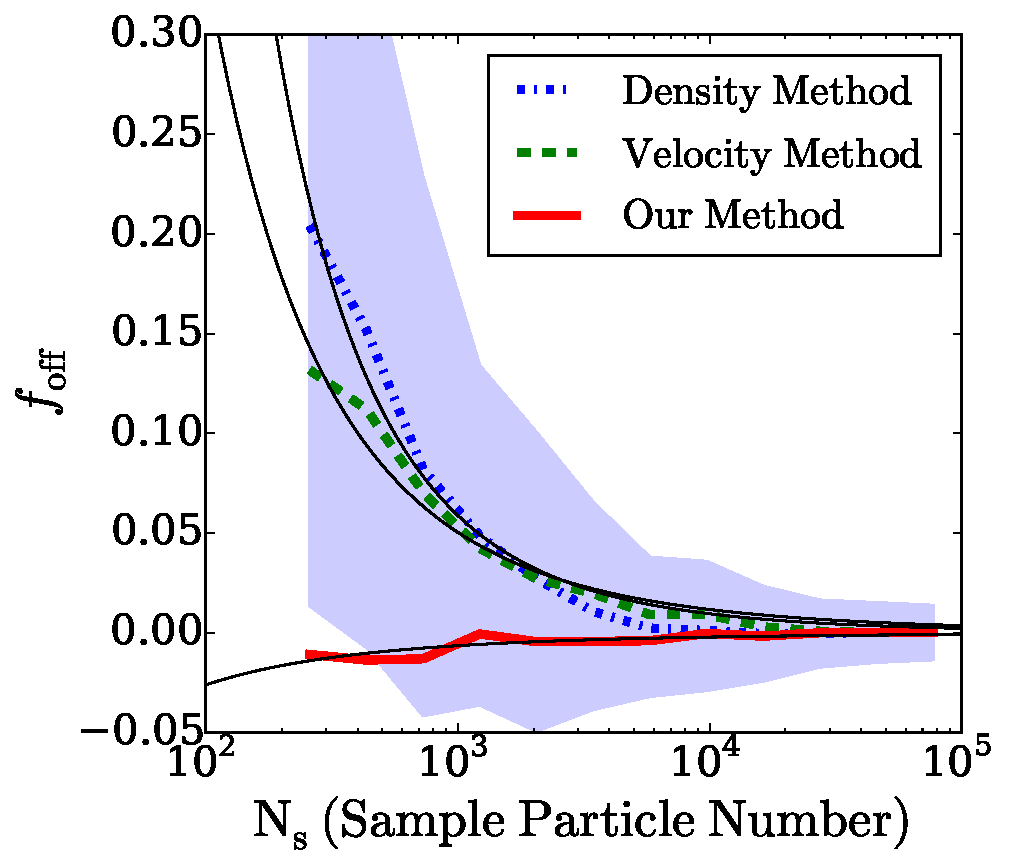
\includegraphics[width=0.49\textwidth]{avg_foff_bolshoi.pdf}
  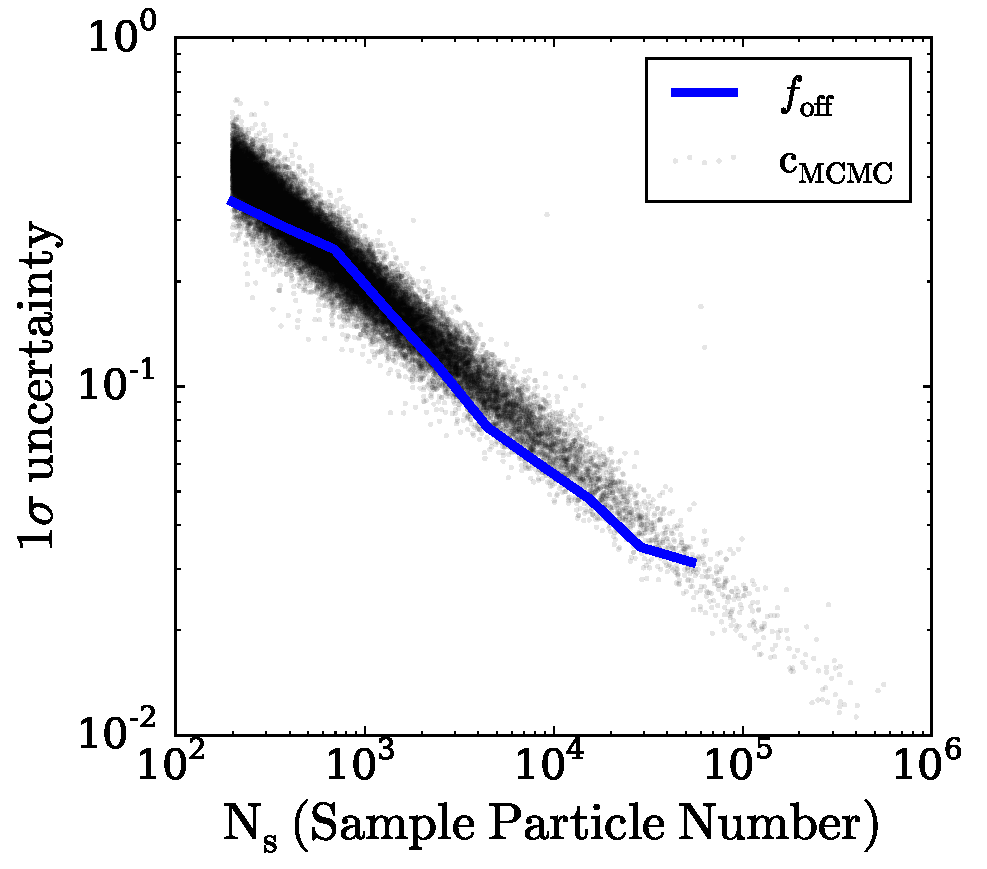
\includegraphics[width=0.48\textwidth]{sigma_foff_bolshoi.pdf}
\end{center}
\vspace{-0.5cm}
\caption{Average value of the fractional offset ($f_{\rm
    off}$Eq. \ref{eq:f_off}) between the concentration in a halo at
  high resolution versus its downsampled versions.  Each point is the
  result of 100 downsampling iterations.  The velocity method
  noticeably overestimates the concentration up to a factor of $0.25$,
  while the new method only underestimates the concentrations by up to
  a factor of $0.05$.
Uncertainties on different concentration estimates.  The
  large symbols show the standard deviation of the fractional offset
  ($f_{\rm off}$ as defined in Eq. \ref{eq:f_off}) from the downsampling
  experiments.  The small dots correspond to the $1\sigma$
  uncertainty on the concentration for each halo as estimated by the
  MCMC algorithm used for the new method.
  The solid lines shows the $1/N$ tendency, which also corresponds
  to the particle number dependence of the $\langle|D|\rangle$ statistic
  (i.e. the accuracy to retrieve a known concentration in mock halos)
  of the new method.
  Uncertainties due to particle number fluctuations are always larger
  than the statistical uncertainties from the fitting process. 
    \label{fig:downsampling}}
\end{figure*}



\section{Methods to estimate the concentration from N-body simulations}
\label{sec:method}

\subsection{Estimates from the density and velocity profiles}

To date, there are two standard methods to estimate concentrations in
dark matter halos extracted from N-body simulations.  The first method
tries to directly estimate the density profile.  It takes all the
particles in the halo and bins them in the logarithm of the radial
coordinate from the halo center.  Then, it estimates the density in
each logarithmic bin counting the particles and dividing by the
corresponding shell volume.  At this point is possible to make a
direct fit to the density as a function of the radial coordinate.
This method has been broadly used for more than two decades to study
the mass-concentration-redshift relation of dark matter halos.
 
A second method uses the circular velocity profile.  It finds the
value of $x$ for which the normalized circular velocity $v(<x)$ shows
a maximum.  Using this value it solves numerically for the
corresponding value of the concentration using Eq. (\ref{eq:max_v}).
This method has been most recently used by \cite{Klypin2016} to study
the mass-concentration-redshift relation using the Multidark
Simulation Suite.


\subsection{Our proposal: estimate from the integrated mass profile}

The new method uses the integrated mass profile defined in
Eq. (\ref{eq:profile}).  We build it from N-body data following the
next steps.  First, we define the center of the halo to be at the
position of the particle with the lowest gravitational potential.
Then we rank the particles by their increasing radial distance from
the center.  From this ranked list of $i=1,N$ particles, the total
mass at a radius $r_i$ is $M_i=i\times m_p$, where $r_i$ is the
position of the $i$-th particle and $m_p$ is the mass of a single
computational particle.  In this process we discard the particle at
the center.

We divide the enclosed mass mass $M_i$ and the radii $r_i$ by their
virial values to obtain the dimensionless variables $m_i$ and $x_i$.
Once the mass profile is expressed in dimensionless variables the
concentration is the only free parameter.  We then use an Affine
Invariant Markov Chain Monte Carlo implemented in the python module
{\texttt{emcee}} \citep{emcee} to sample the likelihood function
distribution defined by ${\cal L}(c)\propto \exp(-\chi^2(c)/2)$ where
the $\chi^2(c)$ is written as

\begin{equation}
\chi^2(c)= \sum_{i=1}^{N}[\log m_i - \log m(< x_i;c)]^2,
\end{equation}
%
where $m(<x_i;c)$ corresponds to the values in Eq.(\ref{eq:profile})
at $x=x_i$ for a given value of the concentration parameter $c$ and
the $i$ index sums over all the particles in the numerical profile.
From the $\chi^2$ distribution we find the optimal value of the
concentration and its associated uncertainty.


\section{Numerical Simulations and Halo Samples}



We use data from the Bolshoi cosmological simulation that follows the
non-linear evolution of a dark matter density field sampled with
$2048^3$ particles over a cubic box of $250\ \hMpc$ on a side.  
The cosmological parameters use a Hubble parameter $h=0.73$, a matter density
$\Omega_m=0.3071$ and a normalization of the power spectrum
$\sigma_8=0.82$. 
The
data is publicly available at \url{http://www.cosmosim.org/}.  More
details about the structure of the database and the simulation can be
found in \citep{2013AN....334..691R}.

We use a halo sample containing all the halos located in a cubic
sub-volume of $100$ \hMpc\ on a side.  From this sample we select all
the halos at $z=0$ detected with a Friends-of-Friends (FoF) algorithm
with more than 300 particles, meaning that the masses are in the
interval $4\times 10^{10}\leq M_{\rm FoF}/\hMsun \leq 10^{14}$.  The
FoF algorithm used a linking length of $0.17$ times the mean
inter-particle distance. This choice translates into an overdensity
$\Delta_h\sim 400-700$ dependent on the halo concentration
\citep{More2011}.

From this set of particles we follow the procedure spelled out in
Section \ref{sec:method} with $\Delta_h=740$ (corresponding to $200$
times the critical density) to select an spherical region that we
redefine to be our halo.  This choice makes that the overdensities are
fully included inside the original FoF particle group.  On the
interest of providing a fair comparison against the density method we
only report results from overdensities with at least $200$ particles
($2.6\times 10^{10}$\hMsun).

We also use public data from the Via Lactea simulation project
\citep{2008Natur.454..735D}.  
This simulation was run for a single isolated halo with a virial mass
of the order of $10^{12}$\hMsun using the parallel tree code PKDGRAV
\citep{2001PhDT........21S}.  
The simulation used $\sim 2\times 10^{8}$ particles to resolve this
region.
The cosmological parameters are diffferent from those in the Bolshoi
simulation, with a Hubble parameter $h=0.73$, a matter density
$\Omega_m=0.238$ and a normalization of the power spectrum
$\sigma_8=0.74$. 
The data available to the public corresponds to a downsampled set 
of $10^5$ particles which corresponds to a particle mass of
$2.24\times 10^{7}$\hMsun.  


We use a set of two very different simulations to demonstrate that the 
results of our bootstraping tests are independent of the kind of
parent simulation.



\begin{figure*}
\begin{center}
  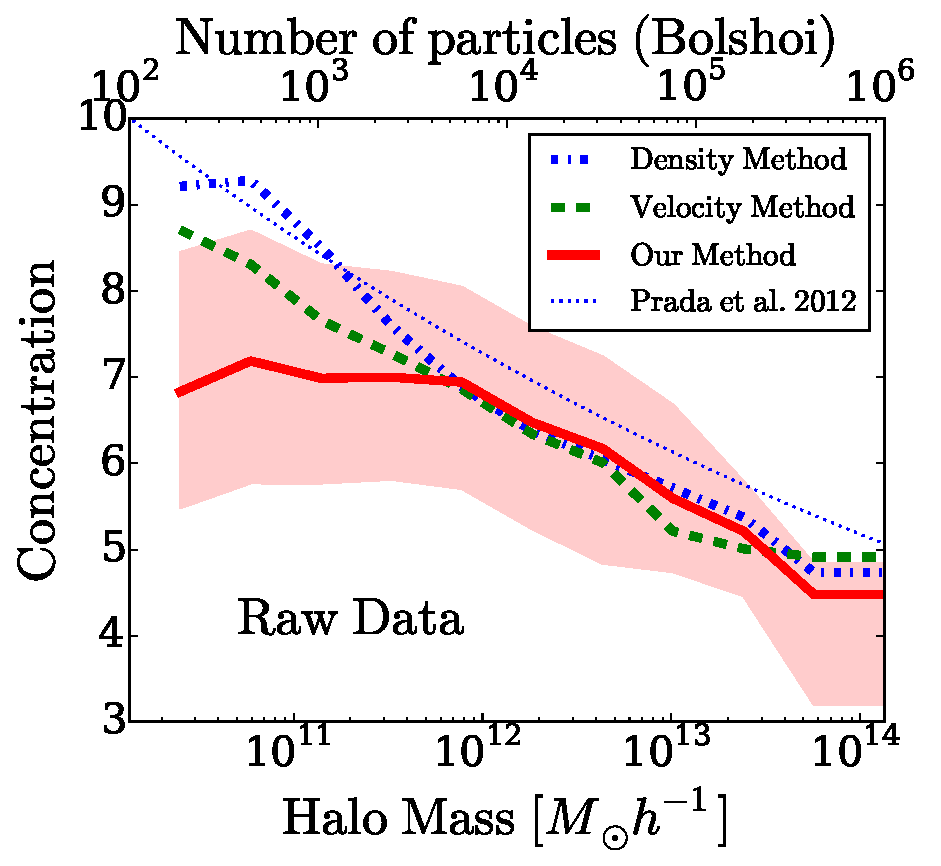
\includegraphics[width=0.49\textwidth]{concentration_bolshoi.pdf}
  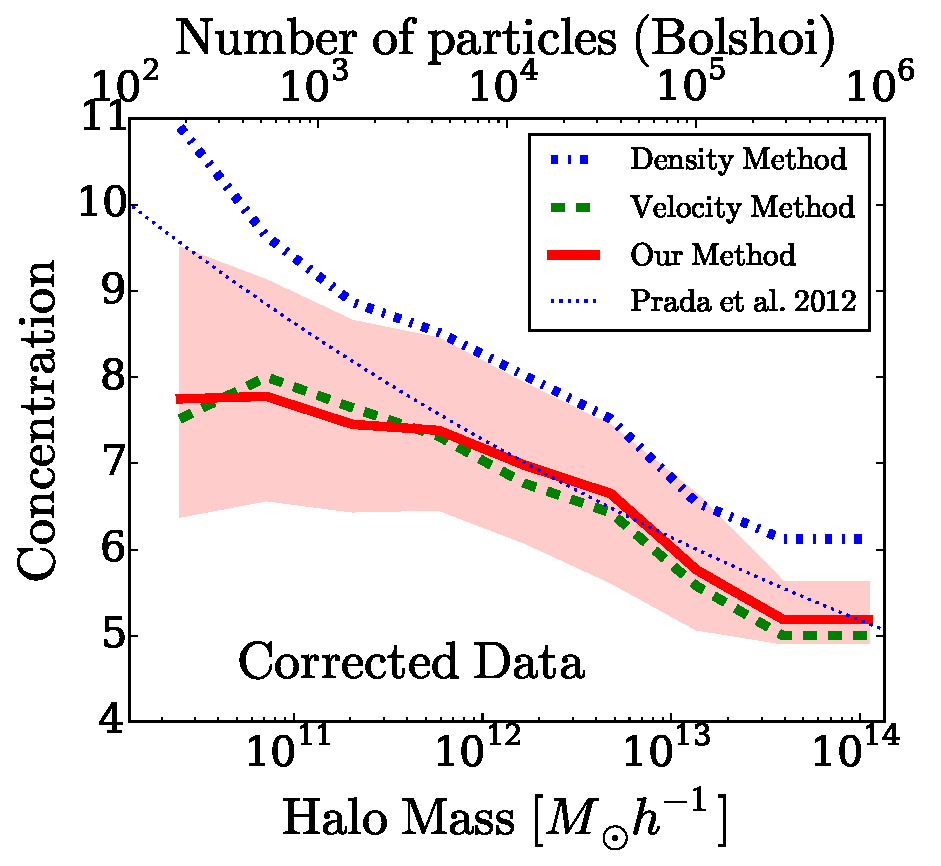
\includegraphics[width=0.49\textwidth]{concentration_bolshoi_corrected.pdf}
\end{center}
\vspace{-0.5cm}
\caption{Mass-concentration relationship for the three different
  methods used on the same cosmological N-body data.  All halos are
  used regardless of their relaxation state.  The lines correspond to
  the median concentration values in each mass bin.  The shaded region
  presents 10 and 90 per cent spread.  For clarity we only show the
  spread for the concentrations estimated using the new method. The
  other two methods have a similar spread. The dotted line corresponds
  to fits reported by \citep{Prada2012}.
  \label{fig:concentration}. The left panel shows the raw results
  coming from each algorithm. The right panel introduces a
  correction on the velocity and integrated mass results. 
  The corrections depends on the number of particles following the
  results of the downsampling experiments presented in Figure
  \ref{fig:downsampling}.} 
\end{figure*}


\section{Results}
\label{sec:results}

\subsection{Bootstrapping to estimate biases}
\label{sec:bootstrapping}

We use bootstraping of individual high resolution halos to quantify
biases for different methods used to esteimate concentrations. 

In this experiment we take halos sampled with at least $10^{5}$
particles and subsample each halo by factors of $2$ up to $10^{3}$ to
measure the concentration every time the halo is resampled.

The average concentration value for the largest number of particles,
$c_{N_{max}}$, provides with a baseline to compare all the other
results.  
We use the following statistic
\begin{equation}
f_{\rm off} = c_{N} / c_{N_{max}} - 1,
\label{eq:f_off}
\end{equation}
to account for the offset between the concentration at a given
downsampled particle number $c_{N}$ and the baseline $c_{N_{max}}$.




We select $8$ halos from the simulation that have at
least $3\times 10^5$ particles.  
We then randomly downsample the total number of particles in each halo
by factors of $10, 20, 45, 100, 215, 460, 1000$ to measure its
concentration with both the integrated mass and the velocity
method. For each downsampling factor we repeat the operation $100$
times.  


Figure \ref{fig:downsampling} summarizes our results.  The plot shows
the average value of $f_{\rm off}$ as a function of the particle
number.  As expected for large enough sample particle numbers,
$N_{s}>5\times 10^3$, the results of the two algorithms coincide and
$\langle f_{\rm off}\rangle\sim 0$.  For lower number of particles,
the results of the two algorithms deviate from the expected
concentration value.  The velocity method overestimates by a factor
$\langle f_{\rm off}\rangle\sim 0.25$ the concentration values for the
lowest sample particle numbers, $N_{s}\sim 100$.  Around the same
sampling scale, the new algorithm shows a more stable behaviour with
an underestimate by a factor of $\langle f_{\rm off}\rangle \sim 0.02$.
This shows that in the more complex setup of a cosmological 
  simulation the new algorithm continues to be stable below the $5\%$
level for low particle numbers.

The line on the same panel shows a fit to the data with the following
functional form 
\begin{equation}
f_{\rm off} = \frac{A}{(1+\log_{10}N_s)^{B}}.
\label{eq:f_off_fit}
\end{equation} 
for the dataset shown in the panel we have $A=3385\pm 2065$, $B=7.99\pm0.48
$ for the velocity method and $A=-110\pm 253$, $B=7.11\pm1.80$ for the
new method, where the uncertainties are estimated from the covariance 
matrix resulting from the non-linear optimization procedure. The lines
on Figure \ref{fig:downsampling} are plotted using these best values. 


Figure \ref{fig:downsampling_err} summarizes different uncertainty
results.  
Large symbols show the standard deviation on $f_{\rm off}$ from the
downsampling experiment.  
Small dots show the uncertainty on each individual concentration value
as estimated by the MCMC algorithm. 
The line shows the $\propto N^{-1}$ locus.  
This figure demonstrates that the statistical uncertainties are at
least one order of magnitude smaller than the uncertainty associated
to downsampling experiment. 


 
\subsection{Impact on the Mass-Concentration Relationship}


Figure \ref{fig:concentration} shows the mass-concentration
relationship for the density, velocity and integrated mass method.
The left panel shows the results as they are produced by each of the
algorithms, the thin dashed line marks the results by
\citep{Prada2012}.

We notice first that the results from the density method have a
systematic $15\%$offset from the velocity methods.  
This offset was already presented by \citep{Prada2012} for low
concentrations ($c<6$) and high ($M_h>10^{12}\hMsun$) halo masses.  
Recently \citep{Klypin2016} summarized results for the
mass-concentration relationship coming from different methods and
datasets to show that similar systematic offsets are present.
\citep{2014MNRAS.441.3359D} studied the mass-concentration
relationship using the maximum velocity and density methods and did
not report any significant difference. However, they implemented a
modified version of the velocity algorithm that uses the data binning
obtained for the density algorithm. 


The new method closely follows the results of
the velocity method at higher masses, $M_h>10^{12}\hMsun$ or
equivalently for $>5\times10^3$ particles.  
For masses below that threshold the new method saturates at a
concentration value of $\sim 8$ while the velocity method continues to
give higher concentration values. 

We hypothesize that the increase in the results for the velocity
method below $5\times 10^{4}$ particles come from the systematic bias
described in the previous subsection.  To test the general consistency
of this hypothesis we correct the concentration values in the
velocity and integrated mass methods by a factor of $1/(1+f_{\rm
  off})$, using the definition in Equation (\ref{eq:f_off}) and the 
parameters obtained from the data presented in Figure
(\ref{fig:downsampling}).  
The correction brings into perfect agreement the results between the
velocity and the integrated mass method.  
This suggests that the concentration at lower masses might very well
reach a plateau in the halo mass range $10^{10}< M_{h}/\hMsun <
10^{12}$ . 


\section{Conclusions}
\label{sec:conclusions}

In this paper we quantified biases on concentration numerical estimates by
bootstrapping dark matter halos resolved with a  large number of
particles ($\sim 10^5$).
We found that methods commonly used in the literature present a large
bias by overestimating concentrations by factors of $13\%$-$20\%$ for
halos with $200$ particles, or $7\%$-$10\%$ for halos with $500$
particles.  
This procedure is a new way to quantify the bias in concentration
estimates with the advantage that it works without having to run new
simulations. 

These results motivated us to introduction a method with a robust
performace at low particle numbers.
This method is based on the integrated mass profile. 
The results of the algorithm on the same data sample showed a bias  of
$2\%-3\%$ for halos with $200$ particles and less than $1\%$ for halos
with $500$ particles or more.  
To keep the bias of the velocity and density methods below $2\%$ only halos
with at least $\sim 4000$ particles should be taken into account.

Measuring the mass concentration relationship the three methods are in
broad agreement within the statistical  uncertainties, although there
are some noticeable differences. 
For instance, the density method produces systematically higher
concentrations by a factor of $15\%$ compared to the velocity method.
This systematic offset has been reported before with the same dataset 
\citep{Prada2012} and with different simulations \citep{Klypin2016}
without any conclusive explanation for its origin. 
A second difference is that the velocity and integrated mass methods
start to differ for masses below $10^{12}\hMsun$.  
We found that correcting the mean concentration by the mean bias
factor brings these two techniques into agreement.

These results show that using the integrated mass profile to find the
Dark Matter halo concentration is a tool deserving deeper scrutiny.   
Further tests with larger simulated volumes, varying numerical
resolution and different density profiles are the next natural step to
explore the full potential of this new method. 


\vspace{0.1cm}

 The authors acknowledge the technical support from the new
 high-performance computing facility at Uniandes. JEF-R acknowledges
 financial support from Vicerrector\'ia de Investigaciones at Uniandes
 through a FAPA project. JCMC acknowledges financial support from
 ``Estrategia de  sostenibilidad 2014-2015, Universidad de
 Antioquia''.    

\bibliographystyle{apj}
%\bibliography{references}
\begin{thebibliography}{15}
\expandafter\ifx\csname natexlab\endcsname\relax\def\natexlab#1{#1}\fi

\bibitem[{{Diemand} {et~al.}(2008){Diemand}, {Kuhlen}, {Madau}, {Zemp},
  {Moore}, {Potter}, \& {Stadel}}]{2008Natur.454..735D}
{Diemand}, J., {Kuhlen}, M., {Madau}, P., {Zemp}, M., {Moore}, B., {Potter},
  D., \& {Stadel}, J. 2008, \nat, 454, 735

\bibitem[{{Duffy} {et~al.}(2008){Duffy}, {Schaye}, {Kay}, \& {Dalla
  Vecchia}}]{Duffy2008}
{Duffy}, A.~R., {Schaye}, J., {Kay}, S.~T., \& {Dalla Vecchia}, C. 2008,
  \mnras, 390, L64

\bibitem[{{Dutton} \& {Macci{\`o}}(2014)}]{2014MNRAS.441.3359D}
{Dutton}, A.~A., \& {Macci{\`o}}, A.~V. 2014, \mnras, 441, 3359

\bibitem[{{Foreman-Mackey} {et~al.}(2013){Foreman-Mackey}, {Hogg}, {Lang}, \&
  {Goodman}}]{emcee}
{Foreman-Mackey}, D., {Hogg}, D.~W., {Lang}, D., \& {Goodman}, J. 2013, \pasp,
  125, 306

\bibitem[{{Klypin} {et~al.}(2016){Klypin}, {Yepes}, {Gottl{\"o}ber}, {Prada},
  \& {He{\ss}}}]{Klypin2016}
{Klypin}, A., {Yepes}, G., {Gottl{\"o}ber}, S., {Prada}, F., \& {He{\ss}}, S.
  2016, \mnras, 457, 4340

\bibitem[{{Ludlow} {et~al.}(2014){Ludlow}, {Navarro}, {Angulo},
  {Boylan-Kolchin}, {Springel}, {Frenk}, \& {White}}]{Ludlow2014}
{Ludlow}, A.~D., {Navarro}, J.~F., {Angulo}, R.~E., {Boylan-Kolchin}, M.,
  {Springel}, V., {Frenk}, C., \& {White}, S.~D.~M. 2014, \mnras, 441, 378

\bibitem[{{Macci{\`o}} {et~al.}(2008){Macci{\`o}}, {Dutton}, \& {van den
  Bosch}}]{Maccio2008}
{Macci{\`o}}, A.~V., {Dutton}, A.~A., \& {van den Bosch}, F.~C. 2008, \mnras,
  391, 1940

\bibitem[{{More} {et~al.}(2011){More}, {Kravtsov}, {Dalal}, \&
  {Gottl{\"o}ber}}]{More2011}
{More}, S., {Kravtsov}, A.~V., {Dalal}, N., \& {Gottl{\"o}ber}, S. 2011, \apjs,
  195, 4

\bibitem[{{Mu{\~n}oz-Cuartas} {et~al.}(2011){Mu{\~n}oz-Cuartas}, {Macci{\`o}},
  {Gottl{\"o}ber}, \& {Dutton}}]{Munoz2011}
{Mu{\~n}oz-Cuartas}, J.~C., {Macci{\`o}}, A.~V., {Gottl{\"o}ber}, S., \&
  {Dutton}, A.~A. 2011, \mnras, 411, 584

\bibitem[{{Navarro} {et~al.}(1997){Navarro}, {Frenk}, \& {White}}]{NFW}
{Navarro}, J.~F., {Frenk}, C.~S., \& {White}, S.~D.~M. 1997, \apj, 490, 493

\bibitem[{{Navarro} {et~al.}(2010){Navarro}, {Ludlow}, {Springel}, {Wang},
  {Vogelsberger}, {White}, {Jenkins}, {Frenk}, \& {Helmi}}]{Navarro2010}
{Navarro}, J.~F., {Ludlow}, A., {Springel}, V., {Wang}, J., {Vogelsberger}, M.,
  {White}, S.~D.~M., {Jenkins}, A., {Frenk}, C.~S., \& {Helmi}, A. 2010,
  \mnras, 402, 21

\bibitem[{{Neto} {et~al.}(2007){Neto}, {Gao}, {Bett}, {Cole}, {Navarro},
  {Frenk}, {White}, {Springel}, \& {Jenkins}}]{Neto2007}
{Neto}, A.~F., {Gao}, L., {Bett}, P., {Cole}, S., {Navarro}, J.~F., {Frenk},
  C.~S., {White}, S.~D.~M., {Springel}, V., \& {Jenkins}, A. 2007, \mnras, 381,
  1450

\bibitem[{{Prada} {et~al.}(2012){Prada}, {Klypin}, {Cuesta}, {Betancort-Rijo},
  \& {Primack}}]{Prada2012}
{Prada}, F., {Klypin}, A.~A., {Cuesta}, A.~J., {Betancort-Rijo}, J.~E., \&
  {Primack}, J. 2012, \mnras, 423, 3018

\bibitem[{{Riebe} {et~al.}(2013){Riebe}, {Partl}, {Enke}, {Forero-Romero},
  {Gottl{\"o}ber}, {Klypin}, {Lemson}, {Prada}, {Primack}, {Steinmetz}, \&
  {Turchaninov}}]{2013AN....334..691R}
{Riebe}, K., {Partl}, A.~M., {Enke}, H., {Forero-Romero}, J., {Gottl{\"o}ber},
  S., {Klypin}, A., {Lemson}, G., {Prada}, F., {Primack}, J.~R., {Steinmetz},
  M., \& {Turchaninov}, V. 2013, Astronomische Nachrichten, 334, 691

\bibitem[{{Stadel}(2001)}]{2001PhDT........21S}
{Stadel}, J.~G. 2001, PhD thesis, UNIVERSITY OF WASHINGTON

\end{thebibliography}


\end{document}


